\documentclass[]{article}

\usepackage[margin=1in]{geometry}

\usepackage[]{amsthm}
\usepackage[parfill]{parskip}
\usepackage[]{graphicx}
\graphicspath{{../img/}}

\newtheorem{theorem}{Theorem}
\newtheorem{lemma}{Lemma}
\newtheorem{corollary}[]{Corollary}

\title{CMSC 510: Dynamic Programming --- Rod Cutting}
\author{Acacia Ackles}

\begin{document}

\maketitle

\section*{Introduction}

We talked about the following process to examine dynamic programming problems.

\begin{enumerate}
    \item Recursion: Come up with a recursive algorithm to solve the problem.
    \item Memoization: Memoize the output from your recursive algorithm so that you can re-access elements
    \item Dynamic Programming: Shift the focus of the problem to the memoized table
\end{enumerate}

See the notes from Ch 14 - Combinations for an example of this process.

In the future, when actually solving dynamic programming problems, you don't need to go through all of these steps; if you recognize it as a problem where dynamic programming may be relevant, you can skip right to coding it up as such. But we're going to walk through these steps to see where they come from. 

\section*{Rod-Cutting Problem}

The book uses Serling Enterprises for this example. I'm using Ackles Steel because my dad owns a steel company and I think it's fun to bring him in on this. 

\subsection*{Informally Stated}

Ackles Steel buys long steel rods and cuts them into shorter rods, which it sells. Each cut is free. Different sized rods have different price points that aren't necessarily directly correlated with size. What's the best way to cut up the rods? 

\subsection*{Formally Stated}

Given a rod of length $n$ inches and a table of prices $p_i$ for $i = 1, 2, \ldots, n$, determine the maximum revenue $r_n$ obtainable by cutting the rod and selling the pieces. If the price of $p_n$ for a rod of length $n$ is large enough, an optimal solution might require no cutting at all. 

\begin{figure}
    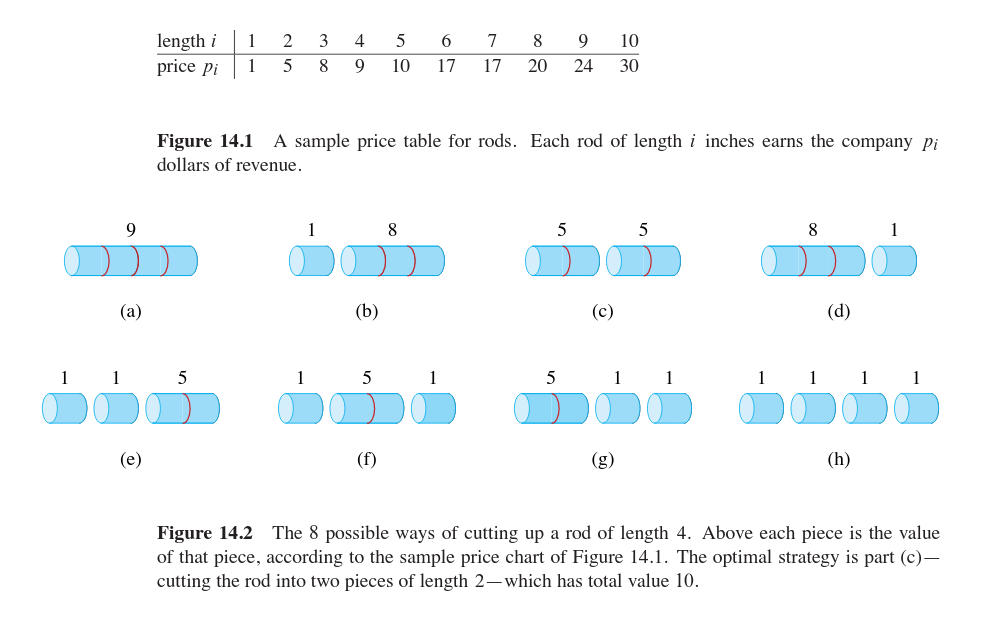
\includegraphics[width=\textwidth]{rod-ex.png}
\end{figure}

\section*{Rod-Cutting Solution}

\subsection*{Analyzing the Problem}

To be able to use dynamic programming or recursion on this problem, we have to find some way to express later solutions in terms of earlier solutions.

If you were asked, what's the maximum possible revenue for a piece of size 1, how would you solve it? What about a piece of size 2? Of size 3?

Generalize to a piece of size $n$. 

\subsection*{Writing a Recursive Solution}

We find that in general, a piece of size $n$ turns the following profit:

$r_n = \max\{p_n, r_1 + r_n-1, r_2 + r_{n-2}, \ldots, r_{n-1} + r_1\}$

Or, in a more condensed format,

$r_n = \max\{p_i + r_{n-i} : 1 \leq i \leq n\}$

What, therefore, will our recursive call look like?

Here is the pseudocode for it:

\begin{verbatim}
    CUT-ROD(p,n):
        if n == 0:
            return 0
    q = -inf
    for i = 1 to n:
        q = max(q, p[i] + CUT-ROD(p, n-i))
    return q
\end{verbatim}

But this takes a long time to run, and if we draw the recursive tree we'll easily see there's a lot of repeats.

\subsection*{Memoization}

We know we are doing a lot of things over and over and over again. So how do we stop doing those things? 

We need to turn this problem into a memoized problem.

Whenever we get a solution, let's save that solution. Simple enough to implement. 

\begin{verbatim}
    CUT-ROD-INIT(p, n)
        let r[0:n] be a new array
        for i = 0 to n
            r[i] = -1
        return CUT-ROD-MEMO

    CUT-ROD-MEMO(p, n, r)
        if r[n] >= 0
            return r[n]
        if n == 0
            q = 0
        else q = -1
            for i = 1 to n
                q = max(q, p[i] + CUT-ROD-MEMO(p, n-i, r))
        r[n] = q
        return q
\end{verbatim}

\subsection*{Dynamic Programming}

Now we want to refocus so that our code basically is surrounding this table rather than having a recursive call itself. 

We do this by constructing a bottom-up approach to the problem.

\begin{verbatim}
     
    let r[0:n] be a new array
    CUT-ROD-DYN(p, n)
        r[0] = 0
        for j = 1 to n:
            q = -1
            for i = 1 to j
                q = max(q, p[i] + r[j-i])
            r[j] = q
        return r[n]

\end{verbatim}

\subsection*{Find the Actual Cuts}

How might you extend this to print not just the revenue, but the actual cuts? 

\begin{verbatim}
     
    let r[0:n] be a new array
    let s[1:n] be a new array
    CUT-ROD-DYN-EXT(p, n)
        r[0] = 0
        for j = 1 to n:
            q = -1
            for i = 1 to j
                if q < p[i] + r[j-i]:
                    q = p[i] + r[j-i]
                    s[j] = i
            r[j] = q
        return r and s

\end{verbatim}

\end{document}